% mnras_template.tex 
%
% LaTeX template for creating an MNRAS paper
%
% v3.2 released 20 July 2023
% (version numbers match those of mnras.cls)
%
% Copyright (C) Royal Astronomical Society 2015
% Authors:
% Keith T. Smith (Royal Astronomical Society)

% Change log
%
% v3.2 July 2023
%	Updated guidance on use of amssymb package
% v3.0 May 2015
%    Renamed to match the new package name
%    Version number matches mnras.cls
%    A few minor tweaks to wording
% v1.0 September 2013
%    Beta testing only - never publicly released
%    First version: a simple (ish) template for creating an MNRAS paper

%%%%%%%%%%%%%%%%%%%%%%%%%%%%%%%%%%%%%%%%%%%%%%%%%%
% Basic setup. Most papers should leave these options alone.
\documentclass[fleqn,usenatbib]{mnras}

% MNRAS is set in Times font. If you don't have this installed (most LaTeX
% installations will be fine) or prefer the old Computer Modern fonts, comment
% out the following line
\usepackage{newtxtext,newtxmath}
% Depending on your LaTeX fonts installation, you might get better results with one of these:
%\usepackage{mathptmx}
%\usepackage{txfonts}

% Use vector fonts, so it zooms properly in on-screen viewing software
% Don't change these lines unless you know what you are doing
\usepackage[T1]{fontenc}

% Allow "Thomas van Noord" and "Simon de Laguarde" and alike to be sorted by "N" and "L" etc. in the bibliography.
% Write the name in the bibliography as "\VAN{Noord}{Van}{van} Noord, Thomas"
\DeclareRobustCommand{\VAN}[3]{#2}
\let\VANthebibliography\thebibliography
\def\thebibliography{\DeclareRobustCommand{\VAN}[3]{##3}\VANthebibliography}


%%%%% AUTHORS - PLACE YOUR OWN PACKAGES HERE %%%%%

% Only include extra packages if you really need them. Avoid using amssymb if newtxmath is enabled, as these packages can cause conflicts. newtxmatch covers the same math symbols while producing a consistent Times New Roman font. Common packages are:
\usepackage{graphicx}	% Including figure files
\usepackage{amsmath}	% Advanced maths commands

%%%%%%%%%%%%%%%%%%%%%%%%%%%%%%%%%%%%%%%%%%%%%%%%%%

%%%%% AUTHORS - PLACE YOUR OWN COMMANDS HERE %%%%%

% Please keep new commands to a minimum, and use \newcommand not \def to avoid
% overwriting existing commands. Example:
%\newcommand{\pcm}{\,cm$^{-2}$}	% per cm-squared

%%%%%%%%%%%%%%%%%%%%%%%%%%%%%%%%%%%%%%%%%%%%%%%%%%

%%%%%%%%%%%%%%%%%%% TITLE PAGE %%%%%%%%%%%%%%%%%%%

% Title of the paper, and the short title which is used in the headers.
% Keep the title short and informative.
\title[How to get energy from a black hole?]{How to get energy from a black hole?}

% The list of authors, and the short list which is used in the headers.
% If you need two or more lines of authors, add an extra line using \newauthor
\author[A. Gorodilov]{
A. Gorodilov,$^{1}$\thanks{E-mail: poruchik\_rzhevsky@physics.muni.cz}
\\
% List of institutions
$^{1}$Department of Theoretical Physics and Astrophysics, Faculty of Science, Masaryk University, Kotlářská 2, 611 37 Brno, Czech Republic
}

% These dates will be filled out by the publisher
\date{Accepted XXX. Received YYY; in original form ZZZ}

% Enter the current year, for the copyright statements etc.
\pubyear{2015}

% Don't change these lines
\begin{document}
\label{firstpage}
\pagerange{\pageref{firstpage}--\pageref{lastpage}}
\maketitle

% Abstract of the paper
\begin{abstract}
This paper discusses the potential energy source for advanced extraterrestrial civilizations, especially those classified as Type III on the Kardashev scale. The primary focus is on a physics-based approach: harnessing energy from Black Hole (BH). The study discusses a model of energy harvesting from BH called the Penrose machine within the framework of general relativity. The results suggest that BH could serve as a powerful and sustainable source of energy for civilizations seeking to expand their influence across galaxies.
\end{abstract}


\begin{keywords}
black holes -- general relativity -- penrose process
\end{keywords}

%%%%%%%%%%%%%%%%%%%%%%%%%%%%%%%%%%%%%%%%%%%%%%%%%%

%%%%%%%%%%%%%%%%% BODY OF PAPER %%%%%%%%%%%%%%%%%%

\section{Introduction}

How can the economy of extraterrestrial civilizations be arranged to provide the energy to conquer new and new galaxies? We can speculate about tachyon generators, energy converters from universes with different physics, or a big furnace burning dark matter. But if we approach the question more realistically, without inventing completely exotic entities, will we have to curl every star into a Dyson sphere \citet{dyson1960}? In fact, there is an energy production mechanism so efficient that it would be worthy of a Type 3 civilization on the Kardashev scale \citet{kardashev1964}. And the source of that energy would be a black hole (BH).

\section{The physics of black holes}

\subsection{Static non-rotating black hole}

No one has yet succeeded in creating a real BH in an experimental facility on Earth. That is why we talk about modelling them based on General Relativity (GR). There are different models. The first and simplest one appeared almost immediately after Einstein's publication of the GR in 1915-1916 and was authored by the German physicist Karl Schwarzschild. He quickly took up the mathematical apparatus of the new theory and quickly found the first exact solution of Einstein's equations \citet{schwarzschild1999}. 

The solution was the simplest, non-rotating and chargeless BH. That is, some region in which space is warped to such an extent that escape from it would require speed greater than the speed of light. The boundary of this region is called the Event Horizon (EH) and is defined by the Schwarzschild radius:

\begin{equation*}
	r_s = \frac{2GM}{c^2}
\end{equation*}

The Schwarzschild metric for the non-rotating uncharged BH in standard Schwarzschild coordinates $(t, r, \theta, \phi)$ is shown in equation~\ref{eq:swarz_metric}. The line element is given in equation~\ref{eq:line_element}.

\begin{equation}
g_{\mu\nu} =
\begin{bmatrix}
	-\left(1 - \frac{2GM}{r}\right) & 0 & 0 & 0 \\
	0 & \left(1 - \frac{2GM}{r}\right)^{-1} & 0 & 0 \\
	0 & 0 & r^2 & 0 \\
	0 & 0 & 0 & r^2 \sin^2 \theta
	\label{eq:swarz_metric}
\end{bmatrix}
\end{equation}

\begin{equation}
	\begin{split}
		ds^2 &= -\left( 1 - \frac{2GM}{r} \right) dt^2 
		+ \left( 1 - \frac{2GM}{r} \right)^{-1} dr^2 \\
		&\quad + r^2 d\theta^2 
		+ r^2 \sin^2 \theta d\phi^2
	\end{split}
	\label{eq:line_element}
\end{equation}

Later, it turned out that BH is not just a mathematical toy. When a massive star collapses after consuming hydrogen it explodes in a supernova. For some combination of the initial mass of the star and the mass of the remnant after the supernova explosion (see Table~\ref{tab:masses}), the compression of the star cannot be stoped and, by all accounts, the whole volume of the remnant should be all at the very center of the BH, at a point where there should theoretically be infinite density and infinite curvature of space and time. Such a point is called a singularity. It turns out that the event horizon is a kind of conditional boundary of the black hole. The radius at which the escape velocity is equal to the speed of light.

\begin{table*} % Single column table
	\centering
    \caption{Evolution of stars by their mass}
    \begin{tabular}{l l r}
        \hline
        Initial mass of the star $[\textup{M}_\odot]$ & Mass of the remnant (core) $[\textup{M}_\odot]$ & Final stage \\
        \hline
        $< 8$  & ---  & White dwarf \\
        $8 - 20$  & $1.4 - 3$ & Neutral star \\
        $20 - 40$  & $> 3$ & Black hole \\
        $> 40$ & Direct collaps & Black hole \\
        \hline
    \end{tabular}
	\label{tab:masses}
\end{table*}

\subsection{Non-static rotating black hole}

Schwarzschild's BH is a somewhat simplified model. In all likelihood, there are no such ideal BHs in the universe. And the reason is the rotation of the stars. The Sun makes a complete rotation on its axis in about $25.67 \text{d}$ (at the equator). More massive stars rotate even faster, and it is the massive stars that are candidates for the role of future black holes. When these stars collapse, their rotation rate increases many times over. This is a consequence of the law of conservation of momentum. For example: if the Sun were to shrink to its Schwarzschild radius of $\approx 3\text{km}$, while fully conserving its torque, it would rotate at up to 1000 revolutions per second, and the speed at the equator would be about 45\% of the speed of light.  

It turns out that the BHs formed by the collapse of stars should rotate, and rotate quite rapidly. But what exactly is rotating in a BH? After all, we're talking about an infinitesimal point in space, what does rotation have to do with it? The BH is described by only three parameters: mass, momentum and electric charge. Momentum is just responsible for rotation, and according to the law of conservation of energy - all these quantities must be conserved, so BH must inherit momentum from the parent star. 

The solution to the GR equations was not obtained until almost 50 years after Schwarzschild's success. It was succeeded in 1963 by Roy Kerr \citet{kerr1963}. The Kerr metric in Boyer-Lindquist coordinates $(t, r, \theta, \phi)$ is represented by the equation~\ref{eq:kerr_metric}.

\begin{equation}
	\begin{split}
		ds^2 &= -\left( 1 - \frac{2GM r}{\Sigma} \right) dt^2 
		- \frac{4GM a r \sin^2\theta}{\Sigma} dt d\phi 
		+ \frac{\Sigma}{\Delta} dr^2 \\
		&+ \Sigma d\theta^2 \quad + \left( r^2 + a^2 + \frac{2GM a^2 r \sin^2\theta}{\Sigma} \right) \sin^2\theta d\phi^2
	\end{split}
	\label{eq:kerr_metric}
\end{equation}

where

\begin{equation*}
	\Sigma = r^2 + a^2 \cos^2\theta, \quad
	\Delta = r^2 - 2GM r + a^2.
\end{equation*}

The rotation of the BH makes the mathematics for the calculation much more complex and the physics of the rotating BH becomes much more varied. Already in the time of Schwarzschild, a phenomenon related to the rotation of bodies was known in GR. The first observational confirmation of the theory was the precession of Mercury's orbit. Mercury's perihelion was constantly shifting. This is usually attributed to the gravitational influence of other celestial bodies. Astronomers even tried to search for a planet inside Mercury's orbit and named it Vulcan \citet{weinstein2014}. However, it was not until Einstein found the solution in 1915 as part of the GR. It turned out that, according to GR, rotating bodies entrain space and time, like a vortex, twists in the direction of the body's rotation. This effect is called the Lense-Thirring effect \citet{pfister2007}. A visual representation is shown in the Figure~\ref{fig:lense-thirring}.

\begin{figure} % Single column figure
	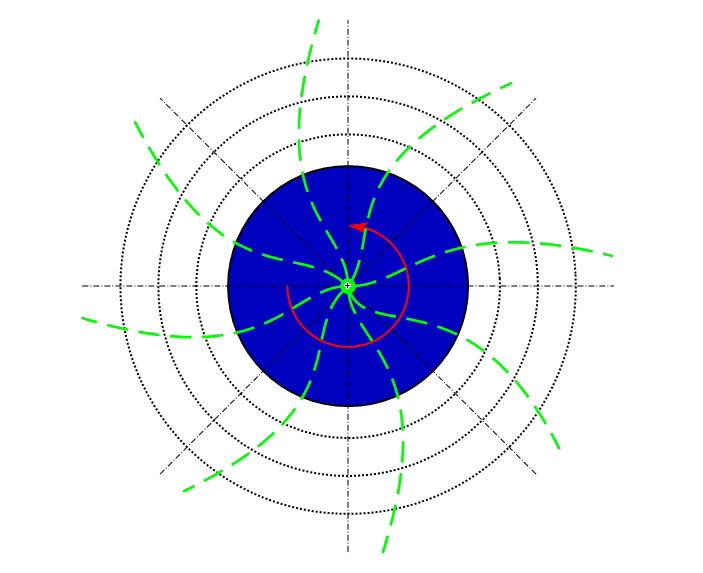
\includegraphics[width=\columnwidth]{figures/lense-thirring.png}
	\caption{Diagram of Frame-dragging effect. Source: \citet{zhang2024}.}
	\label{fig:lense-thirring}
\end{figure}

Static BHs are spherically symmetric. Rotating objects, on the other hand, are stretched in the equatorial region. The EH of a rotating BH, which resembles a rotating ellipsoid, is subject to this effect. Such a BH must have one more important surface, which is called the static limit. It is the limit of space within which the body cannot remain at rest for an external observer. In this region, the body will inevitably curl up into a spacetime vortex in the tension of the BH's rotation. In the non-rotating BH, the EH and the static limit coincide. In rotating BH they touch at the poles. The region between the static limit and the EH is called the ergosphere (see Figure~\ref{fig:ergosphere}). 

\begin{figure} % Single column figure
	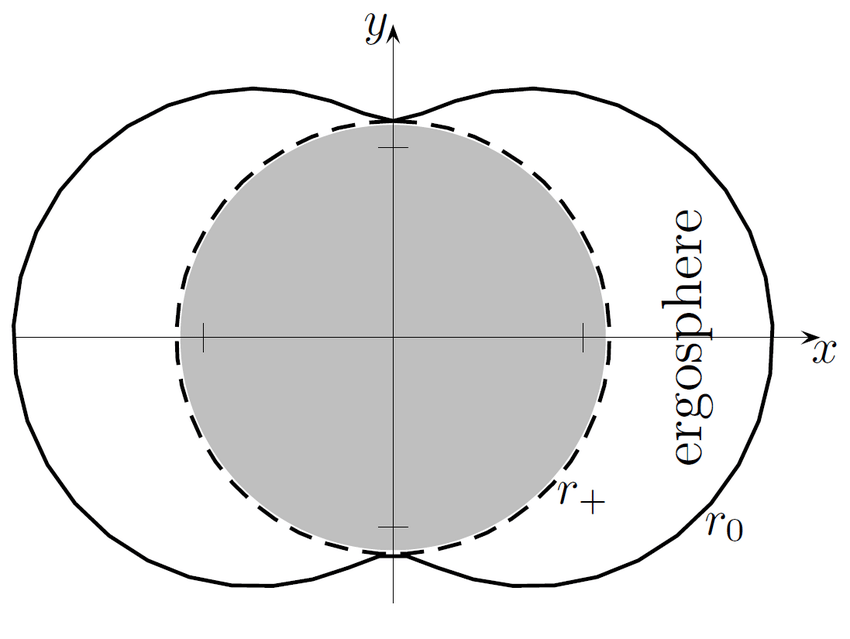
\includegraphics[width=\columnwidth]{figures/ergosphere.png}
	\caption{Event horizon $r_+$ and ergosphere $r_0$ of a rotating Kerr Black Hole. Source: \citet{scharpf2017}.}
	\label{fig:ergosphere}
\end{figure}

\section{Penrose machine}

Once you get past EH, there's no way out. However, it is quite realistic to get into the ergosphere and come back out. In that sense, it works like a carousel: if you join it and then disconnect from it in time, you can gain additional energy through the torque transfer of rotation. At the same time, the BH itself slows down. And that's the principle of energy harvesting. 

In 1969, mathematician Roger Penrose described an interesting property of Kerr's BH \citet{penrose2002}. It turns out that it is not necessary to exert a huge amount of energy on the ergosphere to leave it. It is enough to apply the law of conservation of momentum correctly. Imagine that a body that hits the ergosphere breaks into two parts: one part falls below the EH and is absorbed by the BH, and the other part bounces back and flies out of the BH's immediate vicinity, according to the law of conservation of momentum. If this second part moves with sufficient speed and in the direction of rotation of the BH, it will gain additional energy and momentum due to the rotation of spacetime itself in the ergosphere. The momentum of the BH is transferred to the body. The body accelerates and the rotation of the BH slows down. This process is called the Penrose process (see Figure~\ref{fig:penrose_process}).

\begin{figure} 
	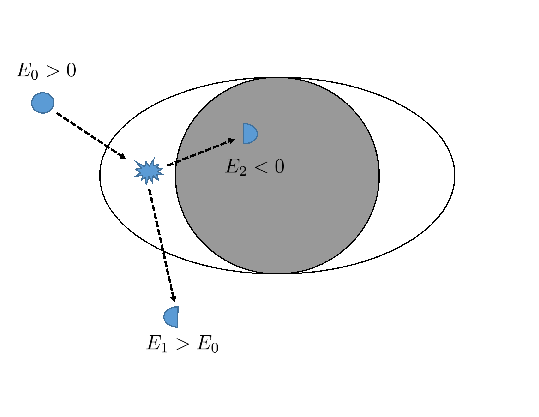
\includegraphics[width=\columnwidth]{figures/penrose_process.png}
	\caption{The Penrose Process. Source: \citet{brito2020}.}
	\label{fig:penrose_process}
\end{figure}

Here comes the simplest idea of a generator based on the Penrose process, the so-called Penrose machine. It is described in \cite{misner1973}. Let us imagine a simple Penrose machine mechanism in the form of a set of carts throwing garbage into the BH (see Figure~\ref{fig:penrose_machine}). Suppose we have a railway platform that moves in a circular path around a rotating BH and is in its ergosphere. On the platform are carts with garbage that can separate and dump some of it inside the EH. When a cart approaches the EH, it splits into two parts: one cart dumps garbage inside the EH and the other is pushed away from it in the opposite direction. There is a region in the ergosphere where a particle can have negative energy relative to an observer at infinity. This means that if the garbage hits the BH with negative energy, the BH will lose some of its rotational energy. The other cart gains additional energy and accelerates, leaving the ergosphere with more velocity than it originally had. As a consequence, the observer at infinity will see that the system has gained additional energy due to the rotation of the BH, without any energy from an external source. Thus, it is possible to periodically launch the cargo carts, throwing some of their mass inside the EH and thus obtaining more and more accelerated carts.

\begin{figure} 
	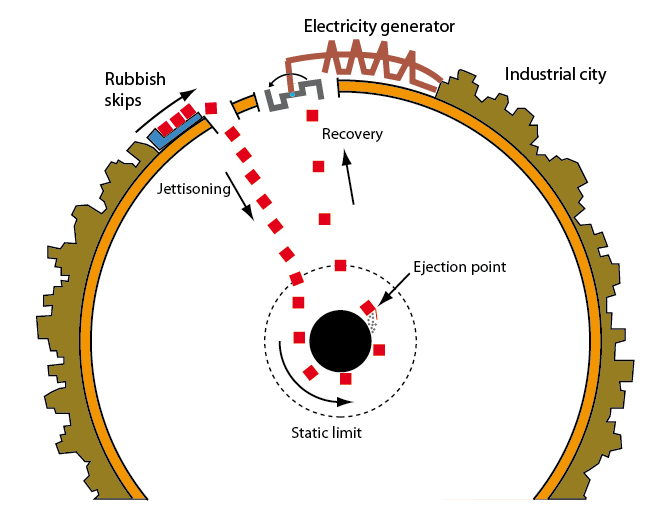
\includegraphics[width=\columnwidth]{figures/penrose_machine.jpg}
	\caption{Industrial extraction of energy from a black hole. Source: \href{https://blogs.futura-sciences.com/e-luminet/2016/01/16/warped-science-interstellar-46-time-dilation-penrose-process/}{The Warped Science of Interstellar (4/6) : Time dilation and Penrose process}.}
	\label{fig:penrose_machine}
\end{figure}

\section{Conclusions}

The use of BH as a source of energy represents a fascinating possibility for advanced civilizations. Theoretical models, including the Penrose process, suggest that rotating BHs can provide significant energy returns. While the experimental creation of BH on Earth remains elusive, their astrophysical counterparts offer a natural environment for energy harvesting. One of the main challenges is to efficiently capture and convert the harvested energy into a usable form without excessive energy losses.

In addition, the construction of structures such as Dyson spheres around BH presents a significant engineering and material challenge. The discussion also touches on the implications of such energy systems for interstellar expansion, particularly in light of potential constraints arising from thermodynamics and quantum effects. Finally, this study highlights the need for further research into the physics of BH and its technological applications, as well as the broader implications for the detection of advanced extraterrestrial civilizations through their energetic signatures.


%%%%%%%%%%%%%%%%%%%%%%%%%%%%%%%%%%%%%%%%%%%%%%%%%%

%%%%%%%%%%%%%%%%%%%% REFERENCES %%%%%%%%%%%%%%%%%%

% The best way to enter references is to use BibTeX:

\bibliographystyle{mnras}
\bibliography{bibliography} % if your bibtex file is called example.bib


% Alternatively you could enter them by hand, like this:
% This method is tedious and prone to error if you have lots of references
%\begin{thebibliography}{99}
%\bibitem[\protect\citeauthoryear{Author}{2012}]{Author2012}
%Author A.~N., 2013, Journal of Improbable Astronomy, 1, 1
%\bibitem[\protect\citeauthoryear{Others}{2013}]{Others2013}
%Others S., 2012, Journal of Interesting Stuff, 17, 198
%\end{thebibliography}

%%%%%%%%%%%%%%%%%%%%%%%%%%%%%%%%%%%%%%%%%%%%%%%%%%


% Don't change these lines
\bsp	% typesetting comment
\label{lastpage}
\end{document}

% End of mnras_template.tex
